\documentclass[11pt]{article}

% Increase main memory size
\usepackage{etex}
\usepackage{morewrites}
\usepackage{multicol}
\usepackage{pgfplots}
\usepackage{tikz}
\usetikzlibrary{external}
\tikzexternalize[prefix=cached_models/]

\usepackage{etex}
\usepackage{morewrites}
\usepackage{enumitem}
\usepackage{float}

\listfiles

\usepackage{amsmath, amssymb, amsthm}
\usepackage{graphicx}
\usepackage{geometry}
\usepackage{array}
\usepackage{booktabs}
\usepackage{float}
\usepackage{verbatim}
\usetikzlibrary{3d}

% Page Layout
\geometry{a4paper, margin=1in}
\setlength\parindent{0pt}
\pgfplotsset{compat=1.18}

% Custom commands
\newcommand{\card}[1]{\lvert #1 \rvert}
\newcommand{\inner}[2]{\left\langle #1, #2 \right\rangle}

\title{\textbf{Exercises in Principles of Mathematical Analysis}}
\author{}
\date{}

\begin{document}

\maketitle

\section*{Exercise 1.1.1}
\textbf{\large Prove that \(\mathbb{Q}\) has zero measure.}

A set \(Q \subset \mathbb{R}\) has measure zero if and only if:
\[Q \subset \bigcup_{j=1}^{\infty} A_j, \quad \text{where } A_j \text{ are intervals and } \sum_{j=1}^{\infty} \card{A_j} < \varepsilon, \forall \epsilon > 0.\]

Since \(\mathbb{Q}\) is countable, we can enumerate its elements as \(\{q_1, q_2, q_3, \ldots\}\). 

We start with:
\[\sum_{j=1}^{\infty} \dfrac{1}{2^{j}} = \dfrac{1/2}{1 - 1/2} = 1.\]

Then, we can multiply this series by any \(\epsilon > 0\) to get:
\[\sum_{j=1}^{\infty} \dfrac{\epsilon}{2^{j}} = \varepsilon.\]

For each rational number \(q_j\), we can construct an interval \(A_j\) centered at \(q_j\) with length \(\dfrac{\varepsilon}{2^{j}}\):
\[A_j = \left(q_j - \dfrac{\varepsilon}{2^{j+1}}, q_j + \dfrac{\varepsilon}{2^{j+1}}\right).\]

Thus, we have:
\[\mathbb{Q} \subset \bigcup_{j=1}^{\infty} A_j, \quad \text{and } \sum_{j=1}^{\infty} \card{A_j} = \sum_{j=1}^{\infty} \dfrac{\varepsilon}{2^{j}} = \varepsilon.\]

Since \(\varepsilon\) can be made arbitrarily small, we conclude that \(\mathbb{Q}\) has measure zero.

\begin{center}
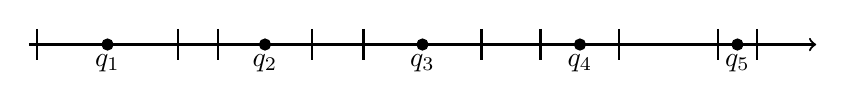
\begin{tikzpicture}
    % Draw the real line
    \draw[thick, ->] (-5, 0) -- (5, 0) node[right] {};
    
    % Place rational points q_i
    \foreach \x/\label in {-4/{$q_1$}, -2/{$q_2$}, 0/{$q_3$}, 2/{$q_4$}, 4/{$q_5$}} {
        \filldraw (\x, 0) circle (2pt) node[below] {\label};
    }
    
    % Draw intervals around q_i as parentheses
    \foreach \x/\len in {-4/0.9, -2/.6, 0/0.75, 2/0.5, 4/0.25} {
        \draw[thick] (\x-\len, 0.2) -- (\x-\len, -0.2);
        \draw[thick] (\x+\len, 0.2) -- (\x+\len, -0.2);
    }
\end{tikzpicture}
\end{center}

\pagebreak
\section*{Exercise 1.1.2}
\textbf{\large For the following function defined on \([0,1]\):
\[f(x) = \begin{cases} 
\dfrac{1}{q} & \text{if } x = \dfrac{p}{q}, \quad p, q \in \mathbb{Z}, q \neq 0 \\
0 & \text{if } x \notin \mathbb{Q}
\end{cases}\]
\begin{enumerate}
    \item Show that \(f\) is discontinuous only at the rational points.
    \item Prove that \(f\) is Riemann integrable.
\end{enumerate}}
\vskip 1em
\begin{center}
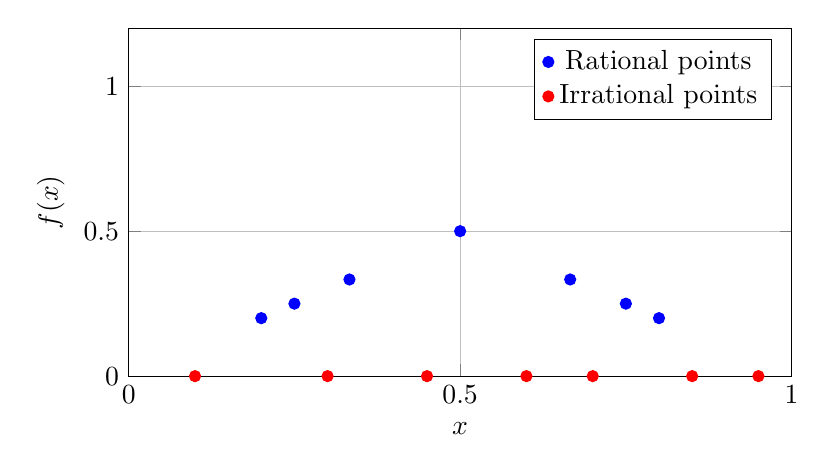
\begin{tikzpicture}
    \begin{axis}[
        width=10cm,
        height=6cm,
        xlabel={$x$},
        ylabel={$f(x)$},
        ymin=0, ymax=1.2,
        xmin=0, xmax=1,
        domain=0:1,
        samples=100,
        ytick={0, 0.5, 1},
        xtick={0, 0.5, 1},
        grid=both,
        legend pos=north east
    ]
        % Plot random points for rationals
        \addplot[only marks, mark=*, color=blue] coordinates {
            (0.2, 1/5) (0.25, 1/4) (0.333, 1/3) (0.5, 1/2) (0.666, 1/3) (0.75, 1/4) (0.8, 1/5)
        };
        \addlegendentry{Rational points}

        % Plot random points for irrationals
        \addplot[only marks, mark=*, color=red] coordinates {
            (0.1, 0) (0.3, 0) (0.45, 0) (0.6, 0) (0.7, 0) (0.85, 0) (0.95, 0)
        };
        \addlegendentry{Irrational points}
    \end{axis}
\end{tikzpicture}
\end{center}

If $x$ is irrational, then
\[\lim_{x \to x_0} f(x) \stackrel{?}{=} 0 = f(x_0),\]

$\forall \varepsilon > 0$, we want $\card{f(x) - 0} = \card{f(x)} < \varepsilon$ if $x$ is close enough to $x_0$ i.e. $x \in \left(x_0 - \delta, x_0 + \delta\right)$ for some $\delta > 0$.

For example, take $\varepsilon = \dfrac{1}{3}$, then $\card{f(x)} < \dfrac{1}{3}$ if $f(x) = \dfrac{1}{q} < \dfrac{1}{3} \Rightarrow q > 3$. So, except for the rationals $0, 1, \dfrac{1}{2}, \dfrac{1}{3}, \dfrac{2}{3}$, we have $\card{f(x)} < \varepsilon = \dfrac{1}{3}$. 
We can do this for any $\varepsilon > 0$ by choosing $q > \dfrac{1}{\varepsilon}$, so 
\[\lim_{x \to x_0} f(x) = 0.\]

So it is continuous at every irrational point. On $\mathbb{Q}$, the value of $f(x)$ is non-zero, so it is discontinuous at every rational point.

Finally, since the set of discontinuities has measure zero ($\card{\mathbb{Q}} = 0$), $f$ is Riemann integrable.

\pagebreak
\section*{Exercise 1.1.4}
\textbf{\large Consider the sequence of functions given by:
\[f_n(x) = \begin{cases}
1 & \text{if } \card{x} \leq n \\
0 & \text{if } \card{x} > n
\end{cases}\]
Obtain the limit \(\lim_{n \to \infty} f_n(x)\) and study whether the convergence is uniform or not.}
\[\sup_{n \in \mathbb{N}} \card{f_n(x) - f(x)} = 1 \neq 0, \quad \forall x \in \mathbb{R}.\]
So the convergence is not uniform.

\section*{Exercise 1.1.5}
\textbf{\large Prove that the following series converges in \([0,1]\). Is the convergence uniform?}
\[\sum_{n=0}^{\infty} x(1 - x)^n = x \sum_{n=0}^{\infty} (1 - x)^n = \begin{cases}
\dfrac{x}{1 - (1 - x)} = \dfrac{x}{x} = 1 & \text{if } x \in (0, 1) \\
0 & \text{if } x = 0 \\
0 & \text{if } x = 1
\end{cases}
\]

If \(\card{1 - x} < 1\), then the series converges. This is true for all \(x \in [0,1]\). The convergence is not uniform since $f$ is not continuous:
\[f_N(x) = \sum_{n=0}^{N} x(1 - x)^n \stackrel{N \to \infty}{\longrightarrow} f(x) = \begin{cases}
1 & \text{if } x \in (0, 1) \\
0 & \text{if } x = 0 \\
0 & \text{if } x = 1
\end{cases}
\]

\section*{Exercise 1.1.3}
\textbf{\large Prove that if a function \(f: [a,b] \to \mathbb{R}\) is monotonus, then it:
\begin{enumerate}
    \item is bounded
    \item is Riemann integrable.
\end{enumerate}}

Suppose \(f\) is monotonically increasing. Then,
\[f(x) \in [f(a), f(b)], \quad \forall x \in [a,b].\]
So \(f\) is bounded.

Now, we build $U_f(P)$ and $L_f(P)$ for a partition $P = \{a, a + \dfrac{b-a}{n}, a + 2\dfrac{b-a}{n}, \ldots, b\}$.
\[U_f(P) = \sum_{i=1}^{n} \sup_{x \in [x_{i-1}, x_i]} f(x) \cdot (x_i - x_{i-1}) = \sum_{i=1}^{n} f(x_i) \cdot \dfrac{b-a}{n},\]
\[L_f(P) = \sum_{i=1}^{n} \inf_{x \in [x_{i-1}, x_i]} f(x) \cdot (x_i - x_{i-1}) = \sum_{i=1}^{n} f(x_{i-1}) \cdot \dfrac{b-a}{n}.\]
Then,
\[U_f(P) - L_f(P) = \dfrac{b-a}{n} \sum_{i=1}^{n} \left(f(x_i) - f(x_{i-1})\right) = \dfrac{b-a}{n} \left(f(b) - f(a)\right) \stackrel{n \to \infty}{\longrightarrow} 0.\]
So \(f\) is Riemann integrable. 

\section*{Exercise 1.1.8}
\textbf{\large Build a sequence of continuous functions on \([0,1]\) that converges to a continuous function, but in a non-uniform way.}
Let us define the sequence of functions:
\[f_n(x) = \begin{cases}
    \sin(n \pi x) & \text{if } x \in \left[0, \frac{1}{n}\right] \\
    0 & \text{if } x \in \left(\frac{1}{n}, 1\right]
\end{cases}
\]
Each \(f_n\) is continuous on \([0,1]\). Now, we find the limit:
\[\lim_{n \to \infty} f_n(x) = 0 = f(x), \quad \forall x \in [0,1].\]
However, the convergence is not uniform. As:
\[\sup_{x \in [0,1]} \card{f_n(x) - f(x)} = \sup_{x \in [0,1]} \card{f_n(x)} = 1, \quad \forall n \in \mathbb{N}.\]

\begin{center}
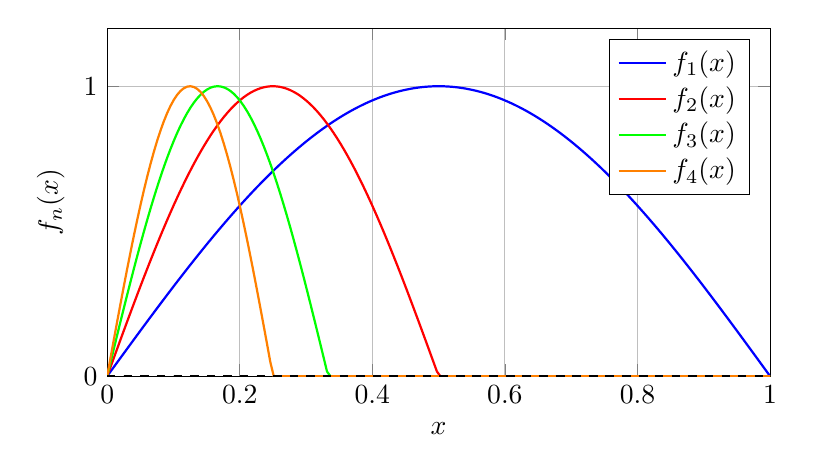
\begin{tikzpicture}
    \begin{axis}[
        width=10cm,
        height=6cm,
        xlabel={$x$},
        ylabel={$f_n(x)$},
        ymin=0, ymax=1.2,
        xmin=0, xmax=1,
        domain=0:1,
        samples=200,
        ytick={0, 1},
        xtick={0, 0.2, 0.4, 0.6, 0.8, 1},
        grid=both,
        legend pos=north east
    ]
        % Plot f_n for n=1,2,3
        \addplot[thick, color=blue] {sin(deg(pi*x))} node[pos=0.8, above] {};
        \addplot[thick, color=red] {x <= 0.5 ? sin(deg(2*pi*x)) : 0} node[pos=0.6, above] {};
        \addplot[thick, color=green] {x <= 0.333 ? sin(deg(3*pi*x)) : 0} node[pos=0.5, above] {};
        \addplot[thick, color=orange] {x <= 0.25 ? sin(deg(4*pi*x)) : 0} node[pos=0.4, above] {};
        \addplot[thick, dashed, color=black] {0} node[pos=0.9, above] {};
        \addlegendentry{$f_1(x)$}
        \addlegendentry{$f_2(x)$}
        \addlegendentry{$f_3(x)$}
        \addlegendentry{$f_4(x)$}

    \end{axis}
\end{tikzpicture}
\end{center}

\section*{Exercise 1.1.9}
\[\lim_{n \to \infty} \int_{-\infty}^{\infty} \dfrac{n^2 - 1}{(x^2 + 1)(n^2 + 1)} \cdot e^{\dfrac{-x^4}{n}} \, dx\]
As \(n \to \infty\),
\[\dfrac{n^2 - 1}{(x^2 + 1)(n^2 + 1)} \cdot e^{\dfrac{-x^4  }{n}} \to \dfrac{1}{x^2 + 1}.\]
So, the limit becomes:
\[\int_{-\infty}^{\infty} \dfrac{1}{x^2 + 1} \, dx = \lim_{N \to \infty} \int_{0}^{N} \dfrac{1}{x^2 + 1} \, dx + \lim_{M \to -\infty} \int_{M}^{0} \dfrac{1}{x^2 + 1} \, dx = \] 
\[= \left[\arctan(x)\right]_{0}^{N} + \left[\arctan(x)\right]_{M}^{0} = \dfrac{\pi}{2} + \dfrac{\pi}{2} = \pi.\]

\pagebreak
\section*{Exercise 1.2.1}
\textbf{\large Let \(f: X \to Y\) be a mapping. Given \(A \subset Y\), let us define:
\[f^{-1}(A) = \{x \in X : f(x) \in A\}.\]
Prove that:}
\begin{enumerate}
    \item \(f^{-1}(Y \setminus A) = X \setminus f^{-1}(A)\).

        If \(x \in f^{-1}(Y \setminus A)\), then \(f(x) \in Y \setminus A\). So, \(f(x) \notin A\), which means \(x \notin f^{-1}(A)\). Thus, \(x \in X \setminus f^{-1}(A)\).

    \item \(f^{-1}\left(\bigcup_{j} A_j\right) = \bigcup_{j} f^{-1}(A_j)\).
    
        If \(x \in f^{-1}\left(\bigcup_{j} A_j\right)\), then \(f(x) \in \bigcup_{j} A_j\). So, there exists some \(j\) such that \(f(x) \in A_j\). Thus, \(x \in f^{-1}(A_j)\) for that \(j\), which means \(x \in \bigcup_{j} f^{-1}(A_j)\).

\end{enumerate}

\section*{Exercise 1.2.2}
\textbf{\large Let \(f : X \to Y\) be a mapping between two topological spaces \((X, \mathcal{T}_X ),
(Y, \mathcal{T}_Y )\). Prove that \(f\) is continuous if and only if \(f\) is continuous at every \(x \in X\).}

For a topological space \((X, \mathcal{T}_X)\), a function \(f: X \to Y\) is continuous if for every open set \(V \in \mathcal{T}_Y\), the preimage \(f^{-1}(V) \in \mathcal{T}_X\).

Now, if \(f\) is continuous at every \(x \in X\), then for every open set \(V \in \mathcal{T}_Y\), we have \(f^{-1}(V) \in \mathcal{T}_X\). Conversely, if \(f\) is continuous, then for every \(x \in X\), and for every open set \(V \in \mathcal{T}_Y\) containing \(f(x)\), we have \(f^{-1}(V) \in \mathcal{T}_X\). Thus, \(f\) is continuous at every \(x \in X\).

\section*{Exercise 1.2.3}
\textbf{\large Show that if \(X = \{1, 2, 3\}\), then \(\mathcal{F} := \{\emptyset, \{2, 3\}, X\}\) is not a \(\sigma\)-algebra.}

To show that \(\mathcal{F}\) is not a \(\sigma\)-algebra, we need to verify the three properties of a \(\sigma\)-algebra:

1. \textbf{Contains the empty set}: \(\emptyset \in \mathcal{F}\).

2. \textbf{Closed under complementation}: The complement of \(\{2, 3\}\) in \(X\) is \(\{1\}\), which \textbf{is not in} \(\mathcal{F}\).
Since \(\mathcal{F}\) is not closed under complementation, it is not a \(\sigma\)-algebra.
\vskip 1em

\section*{Exercise 1.2.4}
\textbf{\large Let \(\mathcal{S}\) be a family of subsets of \(X\), \(S \subseteq \mathcal{P}(X)\). Prove that 
\[\mathcal{A}_\mathcal{S} := \bigcap\{{\mathcal{A} : \mathcal{\mathcal{A}} \text{ is a } \sigma\text{-algebra}, \mathcal{S} \subseteq \mathcal{A}} \subseteq \mathcal{P}(X) \}\]
is the smallest \(\sigma\)-algebra containing \(\mathcal{S}\).}

To prove that \(\mathcal{A}_\mathcal{S}\) is the smallest \(\sigma\)-algebra containing \(\mathcal{S}\), we need to show the following:
\begin{enumerate}
    \item \(\mathcal{A}_\mathcal{S}\) is a \(\sigma\)-algebra. \\
    We know that \(\mathcal{A}_\mathcal{S}\) contains the empty set since every \(\sigma\)-algebra contains the empty set. It is closed under complementation and countable unions because these properties hold for each \(\sigma\)-algebra in the intersection.

    \item \(\mathcal{S} \subseteq \mathcal{A}_\mathcal{S}\). \\
    By definition, \(\mathcal{A}_\mathcal{S}\) is the intersection of all \(\sigma\)-algebras containing \(\mathcal{S}\), so \(\mathcal{S}\) is contained in \(\mathcal{A}_\mathcal{S}\).

    \item If \(\mathcal{B}\) is any \(\sigma\)-algebra containing \(\mathcal{S}\), then \(\mathcal{A}_\mathcal{S} \subseteq \mathcal{B}\). \\
    Since \(\mathcal{A}_\mathcal{S}\) is the intersection of all \(\sigma\)-algebras containing \(\mathcal{S}\), it must be contained in any such \(\sigma\)-algebra \(\mathcal{B}\).
    
\end{enumerate}

Thus, \(\mathcal{A}_\mathcal{S}\) is the smallest \(\sigma\)-algebra containing \(\mathcal{S}\).

\section*{Exercise 1.2.5}
\textbf{\large Let \(X = \{a, b, c, d\}\). Construct the \(\sigma\)-algebra generated by \(E_1 = \{{a}\}\) and by \(E_2 = \{{a}, {b}\}\).}
The \(\sigma\)-algebra generated by \(E_1 = \{a\}\) is:
\[\mathcal{A}_{E_1} = \{\emptyset, \{a\}, \{b, c, d\}, X\}.\]

The \(\sigma\)-algebra generated by \(E_2 = \{a, b\}\) is:
\[\mathcal{A}_{E_2} = \{\emptyset, \{a\}, \{b\}, \{a, b\}, \{c, d\}, \{a, c, d\}, \{b, c, d\}, X\}.\]

\section*{Exercise 1.2.12}
\textbf{\large Let \(u, v : X \to \mathbb{R}\) be measurable functions and let \(\varphi : \mathbb{R} \to \mathbb{R}\) be a continuous function. Prove that}
\begin{enumerate}
    \item \(u + v\), \(uv\) and \(|u|^\alpha\) are measurable.
    \[u + v = \phi(u, v)\]
    \[uv = \phi(u, v)\]
    \[|u|^\alpha = \phi(u)\]
    Every \(\phi\) is continuous, and the composition of measurable functions is measurable. Therefore, \(u + v\), \(uv\), and \(|u|^\alpha\) are measurable.
\end{enumerate}

\section*{Exercise 1.2.13}
\textbf{\large Let \((X, \mathcal{A})\) be a measurable space and let \(f : X \to \mathbb{R}\) be a function. Prove that the following assertions are equivalent:}
\begin{enumerate}
    \item \(\{x \in X : f(x) < \alpha\} \in \mathcal{A}\) for every \(\alpha \in \mathbb{R}\).
    \item \(f^{-1}(B) \in \mathcal{A}\) for every Borel set \(B\). Borel sets on \((\mathbb{R}, \mathcal{T})\) are \(\sigma\)-algebras generated by \(\mathcal{T}\)
\end{enumerate}

We start by proving that (2) implies (1). The open sets \(V \in \mathcal{T}\) are all in \(\mathcal{B}(\mathbb{R})\), so they are all borelians. In (1), we have
\[\{x \in X : f(x) < \alpha\} \stackrel{?}{\in} \mathcal{A}\]
which is equivalent to
\[f^{-1}((\alpha, \infty)), \quad (\alpha, \infty) \in B(\mathbb{R}).\]
Thus, 
\[f^{-1}((\alpha, \infty)) \in \mathcal{A} \text{ by (2).}\]

Now, we prove that (1) implies (2). In \(\mathcal{A}\), since it is a sigma algebra, it must contain \(B(\mathcal{R})\), that is the smallest \(\sigma\)-algebra generated by the open sets. 

\section*{Exercise 1.2.15}
\textbf{\large Prove that if \(f\) is a real function on a measurable space \(X\) such that \(\{x \in X : f(x) \geq r\}\) is measurable for every rational \(r\), then \(f\) is measurable.}
\vskip 1em
We have
\[\forall \alpha \in \mathbb{R}, \quad \exists \{r_n\} \subset \mathbb{Q} : r_n \nearrow \alpha.\]
and \(\{r_n\}\) is increasing (since \(r_n \nearrow \alpha\)). 

\textbf{Note:} \(r_n \nearrow \alpha\) means that \(r_n\) is an increasing sequence that converges to \(\alpha\).
\vskip 1em
We want to prove that
\[f^{-1}((\alpha, \infty)) = \{x \in X : f(x) > \alpha\} \in \mathcal{A}, \quad \forall \alpha \in \mathbb{R}.\]
Consider the increasing sequence \(\{r_n\}\) such that 
\[\lim_{n \to \infty} r_n = \alpha.\]
With this we express
\[(\alpha, \infty) = \bigcap_{n=1}^{\infty} [r_n, \infty)\]
and then
\[\{x \in X : f(x) \geq r\} = f^{-1}((r, \infty)) \in \mathcal{A}, \quad \forall r \in \mathbb{Q}.\]
Thus,
\[f^{-1}((\alpha, \infty)) = f^{-1}\left(\bigcap_{n=1}^{\infty} [r_n, \infty)\right) = \bigcap_{n=1}^{\infty} f^{-1}([r_n, \infty)) \in \mathcal{A}.\]

\section*{Exercise 1.2.16}
\textbf{\large Let \(\mathcal{M}\) be the \(\sigma\)-algebra in \(\mathbb{R}\) given by \(\mathcal{M} = \{\emptyset, (-\infty, 0], (0, \infty), \mathbb{R}\}\). Let \(g\) be the function \(g : \mathbb{R} \to \mathbb{R}\) defined by
\[g(x) = \begin{cases}
0 & \text{if } x \in (-\infty, 0], \\
1 & \text{if } x \in (0, 1], \\
2 & \text{if } x \in (1, \infty).
\end{cases}\]
Is \(g\) measurable? How are the measurable functions \(f : (\mathbb{R}, \mathcal{M}) \to \mathbb{R}\), with the usual topology of the open sets?}

\begin{center}
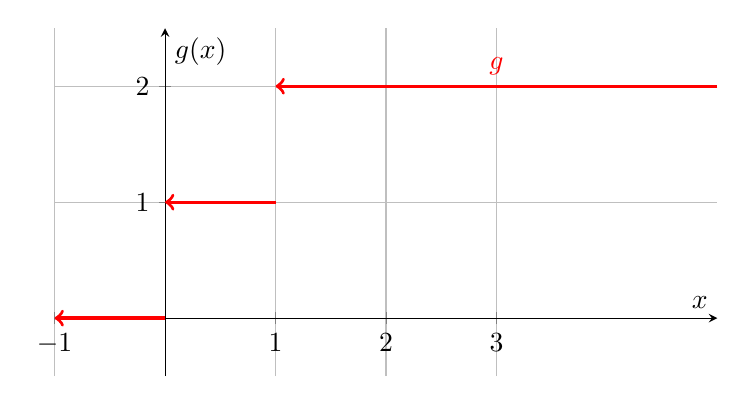
\begin{tikzpicture}
    \begin{axis}[
        width=10cm,
        height=6cm,
        axis lines=middle, 
        xlabel={$x$},
        ylabel={$g(x)$},
        ymin=-0.5, ymax=2.5,
        xmin=-1, xmax=5,
        domain=-1:5,
        samples=200,
        ytick={0, 1, 2},
        xtick={-3, -2, -1, 0, 1, 2, 3},
        grid=both,
        legend pos=north east
    ]
        % Plot g(x)
        \draw[->, very thick, red] (0,0) -- (-1,0);
        \draw[->, very thick, red] (1,1) -- (0,1);
        \draw[->, very thick, red] (5,2) -- (1,2) node[above, pos=0.5] {\(g\)};
    \end{axis}
\end{tikzpicture}
\end{center}

\[\forall V \in \mathcal{T}, \quad g^{-1}(V) \in \mathcal{M}.\]
With \(V = (-1, 3)\), we have \(g^{-1}((-1, 3)) = \mathbb{R} \in \mathcal{M}\).

With \(W = (0, 1)\), we have \(g^{-1}((0, 1)) = \emptyset \in \mathcal{M}\).

With \(H = (-1, 2)\), we have \(g^{-1}((-1, 2)) = (-\infty, 1] \notin \mathcal{M}\).
So \(g\) is not measurable.

\section*{Exercise 1.2.18}
\textbf{\large Let \(\{a_n\}\) and \(\{b_n\}\) be sequences in \(\bar{\mathbb{R}} = [-\infty, \infty]\). Prove that
\begin{enumerate}[label=(\alph*)]
    \item \(\limsup_{n \to \infty} (-a_n) = -\liminf_{n \to \infty} a_n\).
    \item \(\limsup_{n \to \infty} (a_n + b_n) \leq \limsup_{n \to \infty} a_n + \limsup_{n \to \infty} b_n\).
    \item If \(a_n \leq b_n\) for all \(n\), then \(\limsup_{n \to \infty} a_n \leq \limsup_{n \to \infty} b_n\).
    \item Show with an example that strict inequality can hold in part b).
\end{enumerate}}

\textbf{Definition:} If \(\{a_n\}\) is a sequence in \(\bar{\mathbb{R}}\), then the sequence:
\[b_k := \sup \{a_k, a_{k+1}, \ldots\}\]
is decreasing (non-increasing), that is \(b_k \geq b_{k+1}\) for all \(k\). It is bounded from below by \(-\infty\), so it converges to its infimum. The limit is called the \textit{limit superior} of the sequence \(\{a_n\}\) and is denoted by:
\[\limsup_{n \to \infty} a_n = \lim_{k \to \infty} (\sup \{a_k, a_{k+1}, \ldots\})\]

This limit always exists in \(\bar{\mathbb{R}}\). Similarly, consider the sequence:
\[c_k := \inf \{a_k, a_{k+1}, \ldots\}\]
which is increasing (non-decreasing), that is \(c_k \leq c_{k+1}\) for all \(k\). It is bounded from above by \(\infty\), so it converges to its supremum. The limit is called the \textit{limit inferior} of the sequence \(\{a_n\}\) and is denoted by:
\[\liminf_{n \to \infty} a_n = \lim_{k \to \infty} (\inf \{a_k, a_{k+1}, \ldots\}).\]

\subsection*{Example}
Let \(a_n = (-1)^n \arctan(n)\), then
\[\limsup_{n \to \infty} a_n = \lim_{k \to \infty} (\sup \{a_k, a_{k+1}, \ldots\}) = \lim_{k \to \infty} \left(\sup(\arctan(k))\right) = \dfrac{\pi}{2},\]
\[\liminf_{n \to \infty} a_n = \lim_{k \to \infty} (\inf \{a_k, a_{k+1}, \ldots\}) = \lim_{k \to \infty} \left(\inf(-\arctan(k))\right) = -\dfrac{\pi}{2}.\]
So the sequence does not converge, since \(\limsup_{n \to \infty} a_n \neq \liminf_{n \to \infty} a_n\), it does not have a limit.
\vskip 1em
\(\limsup_{n \to \infty} \{a_n\} \) is the largest value for which there is a subsequence converging to it, and \(\liminf_{n \to \infty} \{a_n\} \) is the smallest value for which there is a subsequence converging to it.

\section*{Exercise 1.3.3}
\textbf{\large Let \((X, A)\) be a measurable space and let \(\mu : A \to [0, \infty]\) be a countably additive function on the \(\sigma\)-algebra \(\mathcal{A}\). 
\begin{enumerate}[label=(\alph*)]
    \item Show that if \(\mu\) satisfies that \(\mu(A) < \infty\) for some \(A \in \mathcal{A}\), then \(\mu(\emptyset) = 0\) (and therefore \(\mu\) is a measure).
    \item Find an example for which \(\mu(\emptyset) \neq 0\) (and therefore the countably additivity property does not imply that \(\mu\) is a measure).
\end{enumerate}}

For \(\mu\) to be countably additive, so it must satisfy:
\[\mu\left(\bigcup_{j=1}^{\infty} A_j\right) = \sum_{j=1}^{\infty} \mu(A_j),\]
for any countable collection of disjoint sets \(\{A_j\} \subseteq \mathcal{A}\).

Suppose there exists some \(A \in \mathcal{A}\) such that \(\mu(A) < \infty\). We can express \(A\) as the union of two disjoint sets:
\[A = A \cup \emptyset.\]
By countable additivity, we have:
\[\mu(A) = \mu(A) + \mu(\emptyset).\]
Rearranging this gives:
\[\mu(\emptyset) = \mu(A) - \mu(A) = 0.\]
Thus, if \(\mu\) is countably additive and there exists some \(A \in \mathcal{A}\) with \(\mu(A) < \infty\), then \(\mu(\emptyset) = 0\).

An example where \(\mu(\emptyset) \neq 0\) is the function \(\mu : \mathcal{P}(X) \to [0, \infty]\) defined by:
\[\mu(A) = \begin{cases}
1 & \text{if } A \neq \emptyset, \\
0 & \text{if } A = \emptyset.
\end{cases}\]
This function is not a measure because it does not satisfy \(\mu(\emptyset) = 0\).





\end{document}
